\subsection{Google's License Verification Library (LVL)} \label{section:license-google}
In order to tackle the copy protection problematic and to give the developer community a possibility to fight piracy, Google introduced the \gls{lvl} on the 07/27/2010 \cite{developersLicensingBlog}.
It is easy to use and free of charge.
The documentation can be found on the Android developers website \cite{developersLicensingOverview}.
\newline
Google's approach is based on a network service.
It allows to query the trusted Google Play license server in order to determine whether the user has a valid license.
\newline
\begin{figure}[h]
    \centering
    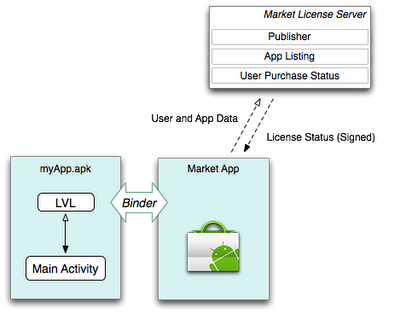
\includegraphics[width=0.5\textwidth]{data/lvl.png}
    \caption{Google's implementation of license checking \cite{developersLicensingOverview}}
    \label{fig:lvl}
\end{figure}
The source code for the \gls{lvl} is provided by Google inside the Android \gls{sdk}.
It has to be manually integrated into the application by the developer.
Since the structure and the way it works can be analysed in the source code, it is vulnerable to attacks.
For this reason, Google instructs the developer to change the library.
Creating an unique implementation by changing its code, structure and control flow to a unique makes it less of a target.
The \gls{lvl} can be integrated in only a few steps.
It is called and based on the result, the normal processing continues or the app terminates.
The logic of the application itself has not to be altered.
\newline
It is necessary to have a Google Publisher Account in order to take advantage of the \gls{lvl}.
It is used to publish applications on the Google Play Store.
The \gls{lvl} does only work when implemented in an application that is distributed in Google's application store and does license verification there.
When an app is registered in Google Developer Console and the entry is created, an application specific public/private key pair is generated.
The use is explained later on. \cite{developersLicensingSetup}
\newline
After an App is registered with the Play Store and the set of keys has been received, \gls{lvl} can be implemented into the application.
The source code of the \gls{lvl} has to be extracted from the Android \gls{sdk} and moved to the application project.
In order to make use of the library inside an application, three extensions to the application's source code have to be made.
 \cite{digipomLvl} \cite{developersLicensingOverview}
\newline
The first extension is the licensing permission in the \textit{AndroidManifest.xml} (see code snippet~\ref{codeSnippet:lvlPermission}).
It is necessary for the \gls{lvl} to work.
When the application tries to contact the server for license verification and the permission is not set, an exception is thrown. \cite{developersLicensingSetup} \cite{developersLicensingAdding}
\newline
\lstinputlisting[
  float=h,
  basicstyle=\footnotesize,
  breakatwhitespace=false,
  breaklines=true,
  captionpos=b,
  frame=single,
  numbers=left,
  language=Java,
  linerange={7-9},
  firstnumber=7,
  caption={Include permission to check the license in AndroidManifest.xml \cite{developersLicensingAdding}},
  label={codeSnippet:lvlPermission}
]{data/permission.xml}
The second extension is the implementation for the asynchronous handling of the callback the license verification call when the process is completed.
The callback has to cover the possible outcomes, \textit{allow()}, \textit{dontAllow()} and \textit{applicationError()}.
The implementation can be seen in code snipped~\ref{codeSnippet:lvlCallback}.
The \textit{applicationError()} is used when the license verification cannot be made, e.g. because no internet connection could be established or because the application is not registered with the Google Play server.
For each of the methods the developer has to implement the code for how the result should be handled. \cite{developersLicensingOverview} \cite{developersLicensingSetup} \cite{developersLicensingAdding} \cite{digipomLvl}
\newline
\lstinputlisting[
  float=h,
  basicstyle=\footnotesize,
  breakatwhitespace=false,
  breaklines=true,
  captionpos=b,
  frame=single,
  numbers=left,
  language=Java,
  linerange={133-149},
  firstnumber=133,
  caption={LVL license check callback},
  label={codeSnippet:lvlCallback}
]{data/lvl.java}
The third extension is the license verification call which can be seen in code snippet~\ref{codeSnippet:lvlSetup}.
The \textit{LicenseChecker}, is initiated by passing three arguments.
The first argument is the application which is provided by Android.
The second argument is the public encryption key.
It is retrieved from the Google Developer console and has to be stored in the code by the developer.
\newline
The third argument is the policy.
The policy decides what happens with the response data, e.g. if it should be cached or requested every time.
The developer has to define the policy.
Google provides two example policies as part of the \gls{lvl}.
Policies require obfuscation to prevent root users from manipulating or reusing the license response data.
An example obfuscator is included in the \gls{lvl}.
It is generated using a salt, the package name and the \textit{ANDROID\_ID}.
The ID is created randomly when the user sets up the device for the first time.
It is unique and remains the same for the lifetime of the user's device.
\newline
When everything is provided, the verification is started by passing  the callback to the \textit{LicenseChecker}'s \textit{checkAcces()} method.
The developer is free to implement the license verification anywhere it is needed.
\cite{developersLicensingOverview} \cite{developersLicensingSetup} \cite{developersLicensingAdding} \cite{digipomLvl}
\newline
\lstinputlisting[
  float=h,
  basicstyle=\footnotesize,
  breakatwhitespace=false,
  breaklines=true,
  captionpos=b,
  frame=single,
  numbers=left,
  language=Java,
  linerange={57-64},
  firstnumber=57,
  caption={Setting up the LVL license check call},
  label={codeSnippet:lvlSetup}
]{data/lvl.java}
Upon execution, the information is passed to the Google Play Service client residing on the device.
The Google Play Service client then adds the primary Google account username and other information and sends the license check request to the server.
On the Google Play server, it is checked whether the user has purchased the application and a corresponding response is send back to the Google Play Service client.
The response is encrypted to ensure integrity and detect tampering.
The Google Play Service client passes it back to the \gls{lvl} which decrypts the response, evaluates it and triggers callback accordingly. \cite{developersLicensingOverview} \cite{developersLicensingSetup} \cite{developersLicensingAdding} \cite{digipomLvl}
\newline
The \gls{lvl} mechanism replaces the old copy protection with a new approach.
Instead of preventing the distribution of the application, the \gls{lvl} prevents the execution of the application.
\newline
It's goal is to provide a simple solution by handling the complicated process, like networking and web services, for the developer.
The developer is in full control of what happens with the response and whether access is granted.
This license verification can be enforced on all devices which have access to Google Play Store and the Google Play Service.
In case the application is installed on a device without the Google Play Service, it cannot bind to it and thus cannot verify the license.
The actual license check obviously requires connection to the internet, as the \gls{lvl} needs to connect to the Google server.
The developer must decide when and how often the license check is done as well as whether the result should be stored for future requests.
Depending on the chosen policy, internet connection is needed. \cite{developersLicensingOverview} \cite{developersLicensingSetup} \cite{developersLicensingAdding} \cite{digipomLvl}
